\documentclass[10pt,a4paper,final]{article}
\usepackage[utf8]{inputenc}
\usepackage[left=2cm,right=2cm,top=2cm,bottom=2cm]{geometry}
\usepackage[hidelinks,]{hyperref}
\hypersetup{colorlinks,
            linkcolor = black,
            urlcolor  = [HTML]{4c72b0},
            citecolor = black,
            anchorcolor = black}
\urlstyle{same}
\usepackage{amsmath}
\usepackage{amsfonts}
\usepackage{amssymb}
\usepackage{graphicx}
\usepackage{array}
\usepackage[table]{xcolor}
\usepackage{tabularx}
\usepackage{ltablex}                    % Tables spanning multiple pages
\usepackage{multirow}
\usepackage{colortbl}
% Definitions of colours used in seaborn for use in latex
\definecolor{seaborn_bg_grey}             {HTML}{eaeaf2}
\definecolor{seaborn_bg_grey_half}        {HTML}{f4f4f8}
 
\definecolor{seaborn_blue}                {HTML}{4c72b0}
\definecolor{seaborn_green}               {HTML}{55a868}
\definecolor{seaborn_red}                 {HTML}{c44e52}
\definecolor{seaborn_magenta}             {HTML}{8172b2}
\definecolor{seaborn_yellow}              {HTML}{ccb974}
\definecolor{seaborn_cyan}                {HTML}{64b5cd}
 
\definecolor{seaborn_muted_blue}          {HTML}{4878cf}
\definecolor{seaborn_muted_green}         {HTML}{6acc65}
\definecolor{seaborn_muted_red}           {HTML}{d65f5f}
\definecolor{seaborn_muted_magenta}       {HTML}{b47cc7}
\definecolor{seaborn_muted_yellow}        {HTML}{c4ad66}
\definecolor{seaborn_muted_cyan}          {HTML}{77bedb}
 
\definecolor{seaborn_pastel_blue}         {HTML}{92c6ff}
\definecolor{seaborn_pastel_green}        {HTML}{97f0aa}
\definecolor{seaborn_pastel_red}          {HTML}{ff9f9a}
\definecolor{seaborn_pastel_magenta}      {HTML}{d0bbff}
\definecolor{seaborn_pastel_yellow}       {HTML}{fffea3}
\definecolor{seaborn_pastel_cyan}         {HTML}{b0e0e6}
 
\definecolor{seaborn_bright_blue}         {HTML}{003fff}
\definecolor{seaborn_bright_green}        {HTML}{03ed3a}
\definecolor{seaborn_bright_red}          {HTML}{e8000b}
\definecolor{seaborn_bright_magenta}      {HTML}{8a2be2}
\definecolor{seaborn_bright_yellow}       {HTML}{ffc400}
\definecolor{seaborn_bright_cyan}         {HTML}{00d7ff}
 
\definecolor{seaborn_dark_blue}           {HTML}{001c7f}
\definecolor{seaborn_dark_green}          {HTML}{017517}
\definecolor{seaborn_dark_red}            {HTML}{8c0900}
\definecolor{seaborn_dark_magenta}        {HTML}{7600a1}
\definecolor{seaborn_dark_yellow}         {HTML}{b8860b}
\definecolor{seaborn_dark_cyan}           {HTML}{006374}
 
\definecolor{seaborn_colorblind_blue}     {HTML}{0072b2}
\definecolor{seaborn_colorblind_green}    {HTML}{009e73}
\definecolor{seaborn_colorblind_red}      {HTML}{d55e00}
\definecolor{seaborn_colorblind_magenta}  {HTML}{cc79a7}
\definecolor{seaborn_colorblind_yellow}   {HTML}{f0e442}
\definecolor{seaborn_colorblind_cyan}     {HTML}{56b4e9}
 

\usepackage[{sf,bf}]{titlesec}
\usepackage{layouts}
\usepackage{calc}
\usepackage[gen]{eurosym}               % Allows euro symbol with \euro
\def\arraystretch{1.5} % Add nicer padding within tables
\renewcommand{\familydefault}{\sfdefault} % Serif
% Setting up tables to by default alternate grey and seaborn_bg_grey_half
\rowcolors{2}{seaborn_bg_grey}{seaborn_bg_grey_half}
\usepackage{longtable}

\author{Edward Linscott}
\title{Marie Curie Part B2}

\begin{document}
   \hbox{%
   \raisebox{-0.535\height}{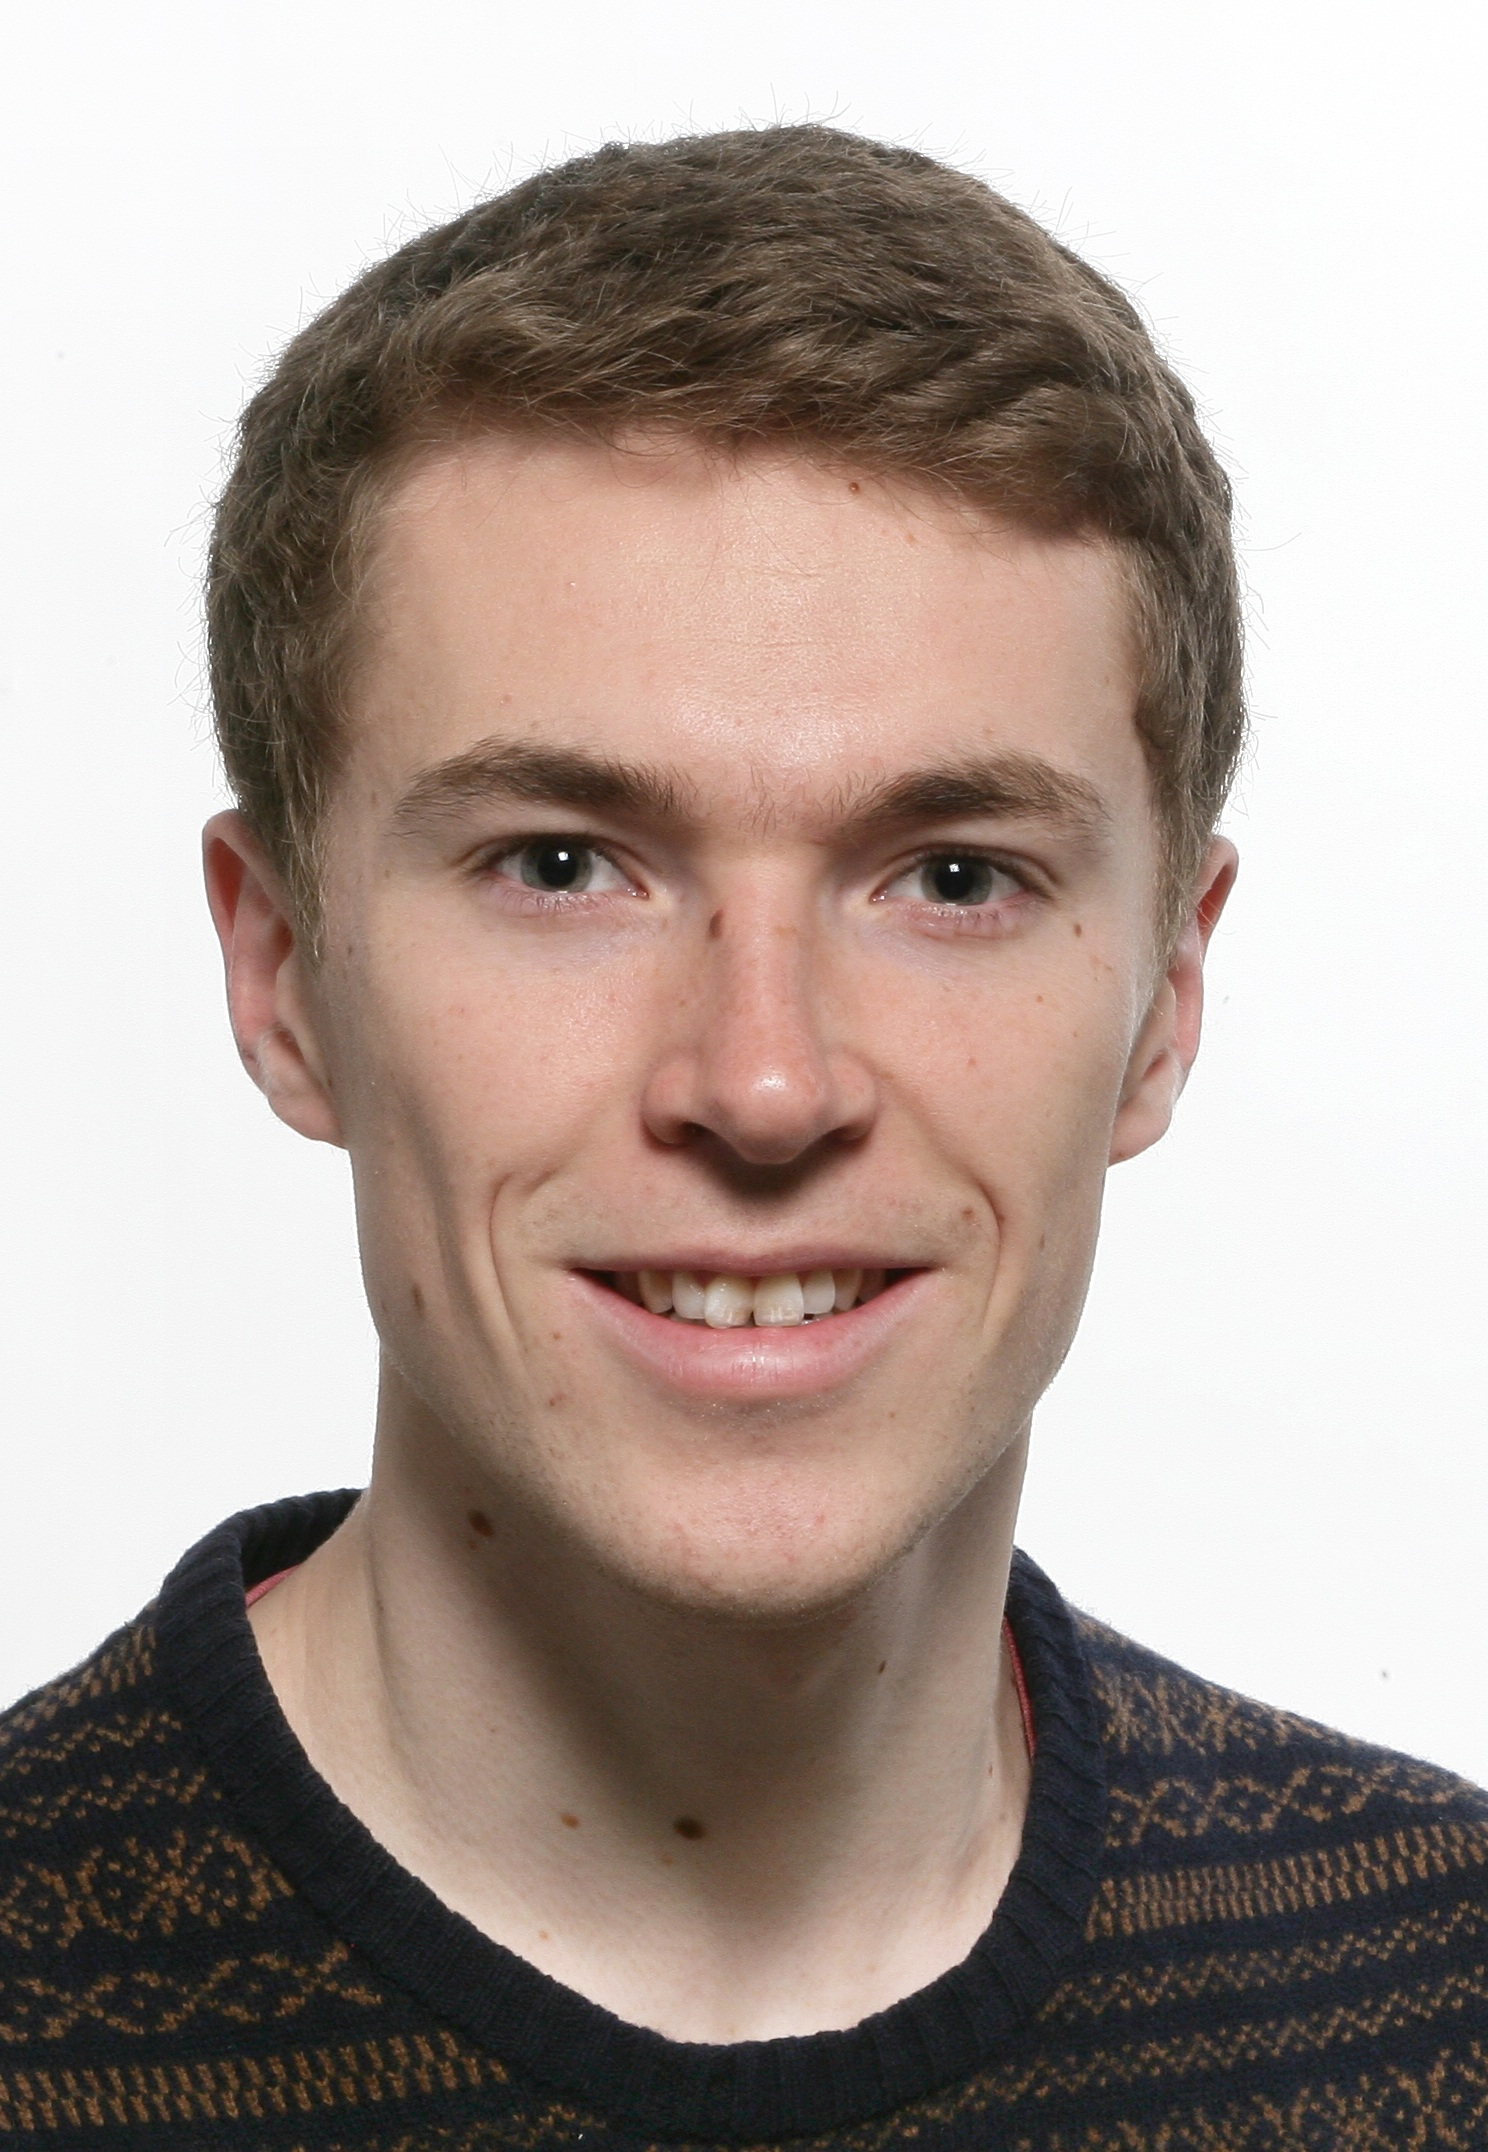
\includegraphics[width=0.12\textwidth]{mugshot.jpg}}%
   \hspace{0.017\textwidth}
   \begin{minipage}{0.856\textwidth}
   \begin{tabularx}{\textwidth}{
         m{\dimexpr0.175\textwidth-2\tabcolsep}%
         m{\dimexpr0.325\textwidth-2\tabcolsep}%
         m{\dimexpr0.175\textwidth-2\tabcolsep}%
         m{\dimexpr0.325\textwidth-2\tabcolsep}}
      \multicolumn{4}{l}{\cellcolor{seaborn_red}}                                                                                   \\[-1.5em]
      \multicolumn{4}{l}{\cellcolor{seaborn_red}%
         \Huge\textbf{\textcolor{seaborn_bg_grey_half}{Edward Linscott}%
         }}                                                                                                                         \\
      \textit{Nationality  } & New Zealander          & \textit{Email  } & edward.linscott@epfl.ch                                  \\
      \textit{Date of birth} & 26/11/1991             & \textit{Phone} & +41 79 678 9641 \\
      \multicolumn{4}{X}{
         
\includegraphics[height=0.7em]{favicons/icons8-google-scholar-192-trimmed.png} \href{https://scholar.google.co.uk/citations?user=4_ejng0AAAAJ}{Google Scholar}
         \quad \quad 
\includegraphics[height=0.7em]{favicons/icons8-github-240-trimmed.png} \href{https://github.com/elinscott}{GitHub}
         \quad \quad 
\includegraphics[height=0.7em]{favicons/icons8-user-90-trimmed.png} \href{https://elinscott.github.io/}{Personal Website}
         \quad \quad 
\includegraphics[height=0.7em]{favicons/icons8-twitter-240-trimmed.png} \href{https://twitter.com/ed_linscott}{Twitter}}
   \end{tabularx}
   \end{minipage}
   }

\begin{tabularx}{\textwidth}{X}
   \cellcolor{seaborn_blue}\large\textbf{\textcolor{seaborn_bg_grey_half}{Summary}} \\
   I am currently a postdoctoral researcher at EPFL in the group of Prof.\ Nicola Marzari. I am researching methods for improving the performance of density functional theory (DFT). Taking inspiration from known properties of the exact functional and our knowledge of the systemic errors of DFT, I (and others) have shown how to construct inexpensive corrections to DFT that drastically improve its performance.

   \vspace{6pt}
   I am now looking for further opportunities where I can apply my expertise in developing density functional approximations and my coding skills to create the next generation of state-of-the-art computational methods for materials science and quantum chemistry.
   
   \vspace{6pt}
   Career highlights thus far include...
   \vspace{6pt}

   -- Receiving (a) the \textit{Prince of Wales Award} for the most outstanding student completing an undergraduate degree at the University of Otago, and (b) the \textit{Cambridge-Rutherford Memorial Scholarship} to enable doctoral studies at the University of Cambridge.
   \vspace{6pt}

   -- Completing a masters and PhD at the University of Cambridge, during which I developed methods and code associated with DFT+\emph{U} and dynamical mean field theory.
    This work has continued during my postdoc with the development of the BLOR functional and a high-throughput study of Hubbard and Hund's parameters.
   \vspace{6pt}

   -- Developing and releasing the \href{https://koopmans-functionals.org/}{koopmans} code, a package that implements Koopmans functionals. I am the lead author of this code. The ``Advanced Quantum ESPRESSO tutorial: Hubbard and Koopmans functionals from linear response'' tutorial in late 2022 covered the use of this code, and had over 200 attendees. % By imposing a generalized piecewise energy condition, these functionals obtain spectral properties with comparable accuracy to GW at a fraction of the computational cost.
   \vspace{6pt}

   -- Supervising Yannick Schubert's master's project and thesis. He said that ``thanks to (Edward's) good choice of topics and guidance... achieving good results felt easy. Working with (Edward) was very motivating and a perfect start to a scientific career''.
   \vspace{6pt}
\end{tabularx}%
\setlength{\fboxsep}{5pt}%
\setlength{\fboxrule}{0pt}%

\begin{tabularx}{\textwidth}{
   m{\dimexpr\textwidth-2\tabcolsep}}
   \cellcolor{seaborn_blue}\large\textbf{\textcolor{seaborn_bg_grey_half}{Research and Education}} \\
   \rowcolor{seaborn_bg_grey_half}
   \hbox{%
   \raisebox{-0.5\height}{
   \begin{minipage}[b]{0.825\linewidth}
   {\large \textbf{École polytechnique fédérale de Lausanne, Switzerland}} \\ \textbf{Postdoctoral researcher (1 Nov 2019 -- present)}
   \end{minipage}
      }
   \raisebox{-0.5\height}{\fbox{
\includegraphics[height=0.7cm]{logos/epfl_trimmed.png}}}
   } \\
   % \rowcolor{seaborn_bg_grey_half}%
   % \hbox{%
   %    \raisebox{-0.5\height}{\fbox{
\includegraphics[height=0.7cm]{logos/epfl_trimmed.png}}}
   %    \raisebox{-0.5\height}{\begin{minipage}[b]{0.7\linewidth}
   %          École polytechnique fédérale de Lausanne \\ Switzerland
   %       \end{minipage}}
   % }
   % \\
   % \rowcolor{seaborn_bg_grey_half}%
   % \textbf{}                                        \\
   \rowcolor{seaborn_bg_grey_half}%
   \textit{Supervisor:} Prof. Nicola Marzari
   \\
   \rowcolor{seaborn_bg_grey_half}%
   The goal of my current postdoc is to drive the ongoing development of Koopmans functionals. To this end, I have been one of the main developers of the \href{https://koopmans-functionals.org/}{koopmans} code, a package that (a) implements Koopmans functionals in \texttt{Quantum ESPRESSO} and (b) automates the various workflows that these functionals require. I also was involved in the development of the BLOR functional, a DFT+\emph{U}-type corrective functional that enforces the flat plane condition on localized subspaces, dispensing with the need for an ad hoc derivation from the Hubbard model.
   \\
   %
   % PhD
   %
   % \rowcolor{seaborn_bg_grey}
   % \hbox{%
   %    \raisebox{-0.5\height}{\fbox{
\includegraphics[height=1cm]{logos/cambridge_trimmed.png}}}
   %    \raisebox{-0.5\height}{\begin{minipage}[b]{0.7\linewidth}
   %          University of Cambridge \\ United Kingdom
   %       \end{minipage}}
   % }                                                                                               \\
   \rowcolor{seaborn_bg_grey}
   \hbox{%
      \raisebox{-0.5\height}{
   \begin{minipage}[b]{0.92\linewidth}
   {\large \textbf{University of Cambridge, United Kingdom}} \\ \textbf{PhD in Physics (1 Oct 2015 -- 26 Oct 2019)}
   \end{minipage}
      }
   \raisebox{-0.5\height}{\fbox{
\includegraphics[height=1cm]{logos/cambridge_trimmed.png}}}
   }
   
   % \textbf{PhD in Physics (1 Oct 2015 -- 26 Oct 2019)}                                             \\
   \cellcolor{seaborn_bg_grey}%
   \noindent \textit{Title:} ``Describing Correlation Effects in Biological Systems"
   \\
   \cellcolor{seaborn_bg_grey}%
   \textit{Supervisors:} Prof. Mike Payne and Dr. Daniel Cole (Newcastle)
   \\
   \cellcolor{seaborn_bg_grey}%
   \textit{Funding:} Cambridge-Rutherford Memorial Scholarship (valued at approx.\ \euro{}150,000; competitively awarded)
   \\
   \cellcolor{seaborn_bg_grey}%
   % Many key reactions in biology are performed by metalloproteins. These systems are a challenge to accurately simulate due to two contrasting reasons. Firstly, the strong correlation present due to the transition metal atoms requires more accurate theories than semi-local DFT. And secondly the ambient protein environment requires explicit treatment of thousands of atoms at the quantum-mechanical level.
   I developed novel approaches within linear-response theory for determining Hubbard and Hund's parameters from first principles for DFT\,+\,\emph{U} calculations. I also developed a dynamical mean-field theory module for the linear scaling package ONETEP. I applied these tools to study (a) photodissociation of carboxy-heme (b) the electronic structure of hemocyanin, and (c) water-to-oxygen conversion performed by the oxygen evolving complex.
   \\
   %
   % Masters
   %
\end{tabularx}

\begin{tabularx}{\textwidth}{
   m{\dimexpr\textwidth-2\tabcolsep}}
   \rowcolor{seaborn_bg_grey}
   \textbf{MPhil in Scientific Computing (1 Oct 2014 -- 30 Sep 2015)}
   \\%
   \rowcolor{seaborn_bg_grey}

   \textit{Title:} ``Strong Correlation Effects in the Electronic Structure of the Photosystem II Complex"
   \\
   \rowcolor{seaborn_bg_grey}%

   \textit{Supervisors:} Prof. Mike Payne and Dr. Daniel Cole
   \\
   \rowcolor{seaborn_bg_grey}%

   \textit{Funding:} EPSRC; LB Wood Scholarship; Douglass D. Crombie Award in Physics
   \\
   \rowcolor{seaborn_bg_grey}

   Designed to lead into my PhD, my masters project motivated the need for models of the oxygen-evolving complex (OEC) that are thousands of atoms in size, and demonstrated that such calculations are feasible with the linear scaling density functional theory code ONETEP. The thesis also explored the DFT\,+\,\emph{U} as a method for treating the correlation present in the OEC core.
   \\
   \rowcolor{seaborn_bg_grey_half}
   \hbox{%
      \raisebox{-0.5\height}{
   \begin{minipage}[b]{0.93\linewidth}
   {\large \textbf{University of Otago, New Zealand}} \\ \textbf{Research Assistant (1 Mar 2014 -- 31 July 2014)}
   \end{minipage}
      }
   \raisebox{-0.5\height}{\fbox{
\includegraphics[height=1cm]{logos/otago_trimmed.png}}}
   }
   % \rowcolor{seaborn_bg_grey_half}
   % \hbox{%
   %    \raisebox{-0.5\height}{\fbox{
\includegraphics[height=1cm]{logos/otago_trimmed.png}}}
   %    \raisebox{-0.5\height}{\begin{minipage}[b]{0.7\linewidth}
   %          University of Otago \\ New Zealand
   %       \end{minipage}}
   % }                                                                                                                                                                                                                                                                                                                                                            \\
   % \rowcolor{seaborn_bg_grey_half}
   % \textbf{Research Assistant (1 Mar 2014 -- 31 July 2014)}                                                                                                                                                                                                                                                                                                     \\
   \cellcolor{seaborn_bg_grey_half}%
   \textit{Supervisor:} Prof. P. Blair Blakie
   \\
   \rowcolor{seaborn_bg_grey_half}
   I was briefly employed as a Research Assistant at the University of Otago, where I continued the work from my honours year studying the behaviour of quasi-2D dipolar Bose-Einstein condensates (BECs). This work resulted in a publication where we predicted an instability of dipolar BECs in regions of experimental interest.                                                          \\
   %
   % Hons
   %
   \rowcolor{seaborn_bg_grey_half} \textbf{BSc (Hons) in Physics (25 Feb 2013 -- 4 Nov 2013)}                                                                                                                                                                                                                                                                   \\
   \cellcolor{seaborn_bg_grey_half}%
   \textit{Title:} ``Non-zero Temperature Theory for Ultra-Cold Dipolar Bose Gases"
   \\
   \cellcolor{seaborn_bg_grey_half}%
   \textit{Supervisor:} Prof. P. Blair Blakie
   \\
   \cellcolor{seaborn_bg_grey_half}%
   \textit{Funding:} University of Otago Prestige Scholarship in Science; Beverley Bursary   \\
   \cellcolor{seaborn_bg_grey_half}%
   \textit{Awards:} Prince of Wales Prize \\
   \cellcolor{seaborn_bg_grey_half}%
   This one-year honours programme was comprised of taught courses in physics and mathematics, and a research project exploring the effects of temperature on the stability of dipolar BECs. I graduated with first-class honours.
   \\
   %
   % BSc
   %
   \rowcolor{seaborn_bg_grey}
   \hbox{%
      \raisebox{-0.5\height}{
   \begin{minipage}[b]{0.815\linewidth}
   {\large \textbf{University of California, Berkeley}} \\ \textbf{Exchange (16 Aug 2012 -- 14 Dec 2012)}
   \end{minipage}
      }
   \raisebox{-0.5\height}{\fbox{
\includegraphics[height=0.8cm]{logos/berkeley_trimmed.png}}}
   }
   \\
   \cellcolor{seaborn_bg_grey}%
   \textit{Funding:} The Alumni of the University of Otago in America Inc. Award \\
   \cellcolor{seaborn_bg_grey}%
   I spent the final semester of my BSc (see below) on exchange at Berkeley.
   \\
   \rowcolor{seaborn_bg_grey_half}
   \hbox{%
      \raisebox{-0.5\height}{
   \begin{minipage}[b]{0.93\linewidth}
   {\large \textbf{University of Otago, New Zealand}} \\ \textbf{BSc in Mathematics and Physics (1 Mar 2010 -- 10 Nov 2012)}
   \end{minipage}
      }
   \raisebox{-0.5\height}{\fbox{
\includegraphics[height=1cm]{logos/otago_trimmed.png}}}
   } \\
   \rowcolor{seaborn_bg_grey_half}
   \textit{Funding:} University of Otago Dux Scholarship; Alumni Annual Appeal Scholarship\\
   \cellcolor{seaborn_bg_grey_half}%
   \textit{Awards:} Robert Jack / Institute of Physics Prize; Gloria Olive Memorial Prize in Mathematics; R. J. T. Bell Prize; New Zealand Institute of Chemistry Prize \\
   \rowcolor{seaborn_bg_grey_half}
   A three-year Bachelor's degree with a double-major in mathematics and physics. I obtained straight A\textsuperscript{+} grades throughout.
   \\
   \rowcolor{seaborn_bg_grey_half}
   \textbf{Summer studentship (21 Nov 2011 -- 30 Jan 2012)}                                                                                                                                                                                                                                                                                                     \\
   \rowcolor{seaborn_bg_grey_half}
   A ten-week studentship in an interdisciplinary research group developing new computed tomography (CT) scanning technology. I wrote code to quantify the quality of their scans.\\
\end{tabularx}
%}

\begin{tabularx}{\textwidth}{l l l l}
   \rowcolor{seaborn_blue}
   \multicolumn{4}{l}{\textcolor{seaborn_bg_grey_half}{\large \textbf{Skills}}}                                                                                                                                                                                                                                                                                                   \\\noalign{\vskip-0.1pt}
   \rowcolor{seaborn_bg_grey}
   \multicolumn{4}{X}{\textbf{\textit{Programming}}                                                                                                                                                                                                                                                                                                                            }             \\\noalign{\vskip-0.1pt}
   \multicolumn{4}{X}{\cellcolor{seaborn_bg_grey}%
   I am a confident programmer, with experience in various languages (including Python and Fortran) and implementing complex algorithms (primarily in the context of electronic structure calculations). I routinely employ good programming practices such as testing, documentation, and CI/CD.
   }                                                            \\\noalign{\vskip-0.1pt}
   
   \multicolumn{4}{X}{\cellcolor{seaborn_bg_grey}%
   Using these skills, I developed \href{https://koopmans-functionals.org}{koopmans}, an open-source package for performing Koopmans functional calculations. I am a contributor to \href{https://www.onetep.org}{ONETEP}, a commercially available scientific DFT code, and I am a developer of TOSCAM, a publically available DMFT code.}       \\\noalign{\vskip-0.1pt}
   \multicolumn{4}{X}{\cellcolor{seaborn_bg_grey}In addition to my formal training in scientific computing, during my PhD I voluntarily attended \href{https://www.cl.cam.ac.uk/teaching/1718/L42/}{\emph{Machine Learning and Algorithims for Data Mining}}, a master's course on machine learning run by the Department of Computer Science and Technology at the University of Cambridge. I also enjoy coding competitions such as \href{https://hashcode.withgoogle.com/}{Google Hash Code}, \href{https://projecteuler.net/}{Project Euler}, and \href{https://www.codingame.com/home}{CodinGame}.}                                                                                                         \\\noalign{\vskip-0.1pt}
   \rowcolor{seaborn_bg_grey}
   \multicolumn{4}{X}{\textit{Languages and interfaces}} \\\noalign{\vskip-0.1pt}
   \rowcolor{seaborn_bg_grey}
   \multicolumn{2}{l}{Used daily}                    & Python, Fortran,  Bash                                                                                                                                                  &                                                                                                                                                                \\\noalign{\vskip-0.1pt}
   \rowcolor{seaborn_bg_grey}
   \multicolumn{2}{l}{Some experience}               & C++, MPI, OpenMP, MATLAB, CUDA                                                                                                                                                      &                                                                                                                                                                \\\noalign{\vskip-0.1pt}
   \rowcolor{seaborn_bg_grey}
   \multicolumn{4}{X}{{\textit{Packages and software}}}                                                                                                                                                                                                                                                                             \\\noalign{\vskip-0.1pt}
   \rowcolor{seaborn_bg_grey}
   \multicolumn{2}{l}{Used daily}                    & \multicolumn{2}{l}{vim, git, vscode, Quantum ESPRESSO, ASE, \LaTeX, SLURM                                                                                                                         }                                                                                                                                                                \\\noalign{\vskip-0.1pt}
   \rowcolor{seaborn_bg_grey}
   \multicolumn{2}{l}{Extensive experience}      & ONETEP, TOSCAM, PyMol                                                                                                                     &                                                                                                                                                                \\\noalign{\vskip-0.1pt}
   \rowcolor{seaborn_bg_grey}
   \multicolumn{2}{l}{Some experience}               & CASTEP, Siesta, Maestro, VMD, spglib, VESTA                                                                                                                                                &                                                                                                                                                                \\\noalign{\vskip-0.1pt}
   \rowcolor{seaborn_bg_grey_half}
   \textbf{\textit{Teaching}}    &                                                                                                       &                                                                 &                                                                                                                                                                \\\noalign{\vskip-0.1pt}
   \rowcolor{seaborn_bg_grey_half}
   2021-23
                                 & \multicolumn{2}{m{0.59\textwidth}}{Lab demonstrator for master's course in atomistic and quantum simulation of materials}
                                 & EPFL                                                                                                                                                                                                                                                                                                                                    \\\noalign{\vskip-0.1pt}
   \noalign{\vskip-0.1pt} \rowcolor{seaborn_bg_grey_half}
   2017
                                 & \multicolumn{2}{m{0.59\textwidth}}{Supervised ten third-year students for thermal and statistical physics}
                                 & University of Cambridge                                                                                                                                                                                                                                                                                                                 \\\noalign{\vskip-0.1pt}
   \rowcolor{seaborn_bg_grey_half}
   2016
                                 & \multicolumn{2}{m{0.59\textwidth}}{Supervised nine second-year students for experimental methods, oscillations, waves, optics, quantum mechanics, and condensed matter}
                                 & University of Cambridge                                                                                                                                                                                                                                                                                                                 \\\noalign{\vskip-0.1pt}
   \rowcolor{seaborn_bg_grey_half}
   2015
                                 & \multicolumn{2}{m{0.59\textwidth}}{Supervised nine first-year students for physics}
                                 & University of Cambridge                                                                                                                                                                                                                                                                                                                 \\\noalign{\vskip-0.1pt}
   \rowcolor{seaborn_bg_grey_half}
   2013
                                 & \multicolumn{2}{m{0.59\textwidth}}{Lab demonstrator and tutor for first-year biological physics}
                                 & University of Otago                                                                                                                                                                                                                                                                                                                     \\\noalign{\vskip-0.1pt}
   \rowcolor{seaborn_bg_grey}
   \multicolumn{4}{X}{\cellcolor{seaborn_bg_grey}\textbf{\textit{Supervision and mentoring}}}                                                                                                                                                                                                                                                                             \\\noalign{\vskip-0.1pt}
   \multicolumn{4}{X}{\cellcolor{seaborn_bg_grey}During my postdoc I supervised Yannick Schubert, a master's student. He said that ``thanks to (Edward's) good choice of topics and guidance... achieving good results felt easy. Working with (Edward) was very motivating and a perfect start to a scientific career.'' One paper has resulted from this work (with a second in preparation).}                                                                                                                                                                                                                       \\*\noalign{\vskip-0.1pt}
   \multicolumn{4}{X}{\cellcolor{seaborn_bg_grey}I also helped Hovan Lee (PhD student from King's College London) with his DMFT calculations on transferrin. A paper resulted from this work, of which I am the last author.}                                                                                                                                        \\*\noalign{\vskip-0.1pt}
   \multicolumn{4}{X}{\cellcolor{seaborn_bg_grey}During the course of my PhD I provided support to two students. I spent a significant amount of time with M.\,A.\,Al-Badri (Masters, and then PhD student from King's College London), teaching him about DMFT and working with him on DMFT calculations on hemocyanin. I have hosted him in Cambridge twice, and visited him at KCL periodically. A paper resulted from this work. I was also the local port-of-call for S. Mansur (PhD student, Cambridge) for support running ONETEP calculations. This work resulted in two publications.}                                                                                                                                                            \\\noalign{\vskip-0.1pt}
   \rowcolor{seaborn_bg_grey_half}
   \textbf{\textit{Grant writing}}    &                                                                                                                                                                        &         &                                                                                                                                                       \\
   \rowcolor{seaborn_bg_grey_half}
   \multicolumn{4}{X}{\cellcolor{seaborn_bg_grey_half}I have written and received several grants (e.g.\ I was awarded an EPSRC capital grant for over 30K EUR of computing hours). I have also assisted with writing grant applications (e.g.\ a Swiss National Science Foundation grant that was awarded approximately 1M EUR and ranked in the top category of all applications).}\\\noalign{\vskip-0.1pt}
   \rowcolor{seaborn_bg_grey}
   \textbf{\textit{Outreach}}    &                                                                                                                                                                        &         &                                                                                                                                                       \\
   \rowcolor{seaborn_bg_grey}
   \multicolumn{4}{X}{\cellcolor{seaborn_bg_grey}I have assisted at several information days at both EPFL and Cambridge, introducing high school students to computational materials science research.}
\end{tabularx}

% \begin{tabularx}{\textwidth}{
%    m{\dimexpr0.10\textwidth-2\tabcolsep}%
%    m{\dimexpr0.70\textwidth-2\tabcolsep}%
%    >{\raggedleft\arraybackslash}m{\dimexpr0.20\textwidth-2\tabcolsep}}
%    \rowcolor{seaborn_blue}
%    \multicolumn{3}{l}{\large\textcolor{seaborn_bg_grey_half}{\textbf{Selected Grants and Scholarships}}}                                                                           \\
%    \textbf{Year} & \textbf{Description}                                                                                                      & \textbf{Approximate value} \\
%    2018          & EPSRC capital grant for computing hours on CSD3, a Tier-2 HPC centre                                                      & \euro30,000                \\
%    {2014}        & \textit{LB Wood Scholarship} to supplement an existing scholarship for postgraduate study in Britain                      & \euro5,500                 \\
%    {2013}        & \textit{Cambridge--Rutherford Memorial Scholarship} for doctorate studies at the University of Cambridge                  & \euro150,000               \\
%                  & \textit{Douglass D. Crombie Award in Physics} for an Otago graduate embarking on doctoral studies overseas                & \euro 4,000                \\
%    {2012}        & \textit{University of Otago Prestige Scholarship in Science} to support honours study                                     & \euro1,000                 \\
%                  & \textit{Beverley Bursary} for study towards physics honours (2011-2013)                                                   & \euro2,000                 \\
%                  % & \textit{The Alumni of the University of Otago in America Inc. Award} to support an academic exchange to the United States & \euro600                   \\
%    {2010}        & \textit{Alumni Annual Appeal Scholarship} for study at the University of Otago                                            & \euro4,000                 \\
%                  & \textit{University of Otago Dux Scholarship} for study at the University of Otago                                         & \euro4,000                 \\
%                  & \textit{University of Canterbury Dux Scholarship} for study at the University of Canterbury (not taken up)                & \euro4,000                 \\
%                  & \textit{University of Canterbury Mathematics Scholarship} for study at the University of Canterbury (not taken up)        & \euro2,500                 \\
%                  % & \textit{University of Canterbury Science Scholarship} for study at the University of Canterbury (not taken up)            & \euro600                   \\
% \end{tabularx}
% 
% \begin{tabularx}{\textwidth}{m{0.1\textwidth-2\tabcolsep} m{0.9\textwidth-2\tabcolsep}}
%    \rowcolor{seaborn_blue}
%    \multicolumn{2}{l}{\large\textcolor{seaborn_bg_grey_half}{\textbf{Awards and Prizes}}}                                                         \\
%    {2016} & \textit{Poster prize} at CCP9 Young Researchers' Event                                                                                \\
%    {2013} & \textit{Prince of Wales Award} for the most outstanding student completing an undergraduate degree at the University of Otago in 2013 \\
%    {2011} & \textit{Robert Jack / Institute of Physics Prize} for the top student in 200-level physics                                            \\
%           & \textit{Gloria Olive Memorial Prize in Mathematics} for the top student in 300-level mathematics                                      \\
%    {2010} & \textit{Department of Mathematics and Statistics Scholarship} for study at the University of Canterbury                               \\
%           & \textit{Robert Jack / Institute of Physics Prize} for the top student in 100-level physics                                            \\
%           & \textit{R. J. T. Bell Prize} for the top student in 200-level mathematics                                                             \\
%           & \textit{New Zealand Institute of Chemistry Prize} for the top student in CHEM111: Molecular Architecture                              \\
%    % \multicolumn{2}{l}{\textbf{\textit{High School}}} \\
%    % {2009} & \textit{Dux} of Cashmere High School\\
%    % & \textit{NCEA Scholarships} in Calculus, Physics, and Chemistry\\
%    % & Top Year 13 student in English, Physics, and Chemistry\\
%    % {2008} & \textit{McCombs Scholarship} for all round excellence and contributions to Cashmere High\\
%    % & Top Year 12 student in English, Art, Physics, Chemistry, and Year 13 Calculus\\
%    % & \textit{NCEA Scholarship} in Calculus
% \end{tabularx}

\begin{tabularx}{\textwidth}{
      m{\dimexpr0.075\textwidth-2\tabcolsep}%
      m{\dimexpr0.57\textwidth-2\tabcolsep}%
      m{\dimexpr0.15\textwidth-2\tabcolsep}%
      m{\dimexpr0.205\textwidth-2\tabcolsep}}
   \rowcolor{seaborn_blue}
   \multicolumn{4}{l}{\large\textcolor{seaborn_bg_grey_half}{\textbf{Selected talks}}}                                              \\
   \textbf{Year} & \textbf{Event}                                                                                      & \textbf{Location} & \textbf{Contribution} \\
   {2022}        & Advanced Quantum ESPRESSO tutorial: Hubbard and Koopmans functionals from linear response & Virtual & Invited talk (\href{https://youtu.be/tgzgs1bp14w}{video}); Tutorial (\href{https://youtu.be/uaHWhCZoDAk}{video}) \\
                 & 9\textsuperscript{th} Time-Dependent Density-Functional Theory Workshop: Prospects and Applications & Benasque          & Invited talk          \\
   {2021}        & Quantum Theory of Materials Seminar                                                                 & Dublin            & Invited talk (\href{https://youtu.be/E_Uu_ujmWS0}{video})         \\
   {2020}
                 & Quantum Fluids in Isolation Seminar Series                                                          & Boston            & Invited talk (\href{https://youtu.be/AI6qFGf1Zcw}{video})         \\
\end{tabularx}
%
% \begin{tabularx}{\textwidth}{X}
%    \rowcolor{seaborn_blue}
%    \multicolumn{1}{l}{\large\textcolor{seaborn_bg_grey_half}{\textbf{Interests}}} \\
%    I am a violinist, and have been a member (and concertmaster) of many orchestras including the New Zealand Symphony Secondary Schools Orchestra, the Christchurch Youth Orchestra, and the Cambridge Musical Society Symphony Orchestra. I love the outdoors and am an avid runner, cyclist, camper, and hiker.%  I enjoy pub quizzes (having run several for my college's postgraduate community)
% \end{tabularx}

\newpage

\begin{tabularx}{\textwidth}{
      m{\dimexpr0.1\textwidth-2\tabcolsep}
      m{\dimexpr0.45\textwidth-2\tabcolsep}
      m{\dimexpr0.45\textwidth-2\tabcolsep}}
   \rowcolor{seaborn_blue}
   \multicolumn{3}{l}{\textcolor{white}{\large \textbf{Referees}}}                                         \\\noalign{\vskip-0.1pt}
                    & \textbf{\textit{Prof. Mike Payne}} & \textbf{\textit{Prof. Nicola Marzari}}   \\\noalign{\vskip-0.1pt}
   \textit{Address} & 
   
   Theory of Condensed Matter
   
   University of Cambridge
  
   19 J J Thomson Avenue

   Cambridge CB3 0HE

   United Kingdom
   &
   Theory and Simulation of Materials

   École polytechnique fédérale de Lausanne

   Route Cantonale

   1015 Lausanne

   Switzerland                              \\\noalign{\vskip-0.1pt}
   \textit{Email}   & mcp1@cam.ac.uk                     & nicola.marzari@epfl.ch                   \\\noalign{\vskip-0.1pt}
   \textit{Phone}   & +44 (0)1223 337254                 & +41 (0)21 693 1129
\end{tabularx}

\begin{tabularx}{\textwidth}{
   X}
   %   m{\dimexpr0.775\textwidth-2\tabcolsep}%
   %   m{\dimexpr0.225\textwidth-2\tabcolsep}}
   \rowcolor{seaborn_blue}
   %\multicolumn{2}{l}{
      \large\textcolor{seaborn_bg_grey_half}{\textbf{Publications}} \\
   %}
   \textbf{EBL}, N.\,Colonna, R.\,De Gennaro, N.\,L.\,Nguyen, G.\,Borghi, A.\,Ferretti, I.\,Dabo, and N.\,Marzari, \href{https://arxiv.org/abs/2302.07759}{\textit{koopmans: an open-source package for accurately and efficiently predicting spectral properties with Koopmans functionals}}. arXiv:2302.07759 (2023)
   \\
   Y.\,Schubert, N.\,Marzari, and \textbf{EBL}, \href{https://doi.org/10.1063/5.0138610}{\textit{Testing Koopmans spectral functionals on the analytically-solvable Hooke's atom}}. J. Chem. Phys. 158 (2023) 144113
   \\
   A.\,Burgess, \textbf{EBL}, and D.\,D.\,O'Regan, \href{https://doi.org/10.1103/PhysRevB.107.L121115}{\textit{A DFT+U type functional derived to explicitly address the flat plane condition}}. Phys. Rev. B. 107 (2023) L121115
   \\
   G.\,C.\,Moore, M.\,K.\,Horton, A.\,M.\,Ganose, M.\,Siron, \textbf{EBL}, D.\,D.\,O'Regan, and K.\,A.\, Persson, \href{https://arxiv.org/abs/2201.04213}{\textit{High-throughput determination of Hubbard U and Hund J values for transition metal oxides via linear response formalism}}. arXiv:2201.04213 (2022) \\
   N.\,Colonna, R.\,De Gennaro, \textbf{EBL}, and N.\,Marzari, \href{https://pubs.acs.org/doi/10.1021/acs.jctc.2c00161}{\textit{Koopmans spectral functionals in periodic-boundary conditions}}. J. Chem. Theory Comput. 18 (2022) 5435                                                                                                                                                                                                                                                                                                                                                                                                                                                                                                                                                                \\ %&                                                 \\
   R.\,De Gennaro, N.\,Colonna, \textbf{EBL}, and N.\,Marzari, \href{https://doi.org/10.1103/PhysRevB.106.035106}{\textit{Bloch's theorem in orbital-density-dependent functionals: Band structures from Koopmans spectral functionals}}. Phys. Rev. B 106 (2022) 035106                                                                                                                                                                                                                                                                                                                                                                                                                                                                                                     \\ % & 1 citation                                      \\
   % 
   H.\,Lee, C.\,Weber, and \textbf{EBL}, \href{https://doi.org/10.1021/acs.jpclett.2c00680}{\textit{Many-body study of Iron (III)-bound human serum transferrin}}. J. Phys. Chem. Lett. 13 (2022) 4419                                                                                                                                                                                                                                                                                                                                                                                                                                                                                                                                                                      \\ % &                                                 \\
   % 
   % 
   R.\,Kobayashi, T\,P.\,M.\,Goumans, N.\,Ole Carstensen, T.\,M.\,Soini, N.\,Marzari, I.\,Timrov, S.\,Ponc\'e, \textbf{EBL}, C.\,J.\,Sewell, G.\,Pizzi, F.\,Ramirez, M.\,Bercx, S.\,P.\,. Huber, C.\,S.\,Adorf, and L.\,Talirz, \href{https://doi.org/10.1021/acs.jchemed.1c00655}{\textit{Virtual computational chemistry teaching laboratories – hands-on at a distance}} J. Chem. Educ. 98 (2021) 3163                                                                                                                                                                                                                                                                                                                                                                  \\ %& 8 citations                                     \\
   % 
   \textbf{EBL}, D.\,J.\,Cole, N.\,D.\,M.\,Hine, M.\,C.\,Payne, and C.\,Weber, \href{https://doi.org/10.1021/acs.jctc.0c00162}{\textit{ONETEP + TOSCAM: uniting dynamical mean field theory and linear-scaling density functional theory}} J. Chem. Theory Comput. 16 (2020) 4899                                                                                                                                                                                                                                                                                                                                                                                                                                                                                          \\ %& 5 citations                                     \\
   S.\,M.\ Masur, \textbf{EBL}, and C.\,J.\ Edgcombe, \href{https://www.sciencedirect.com/science/article/pii/S036820481930221X}{\textit{Modelling a capped carbon nanotube by linear-scaling density-functional theory}}, J. Electron Spectrosc. Relat. Phenom. 241 (2020) 146896                                                                                                                                                                                                                                                                                                                                                                                                                                                                                     \\ %& 3 citations                                     \\
   J.\,C.\,A.\ Prentice, J.\ Aarons, J.\,C.\ Womack, A.\,E.\,A.\ Allen, L.\ Andrinopoulos, L.\ Anton, R.\,A.\ Bell, A.\ Bhandari, G.\,A.\ Bramley, R.\,J.\ Charlton, R.\,J.\ Clements, D.\,J.\ Cole, G.\ Constantinescu, F.\ Corsetti, S.\,M-M.\ Dubois, K.\,K.\,B.\ Duff, J.\ María Escartín, A.\ Greco, Q.\ Hill, L.\,P.\ Lee, \textbf{EBL}, D.\,D.\ O’Regan, M.\,J.\,S.\ Phipps, L.\,E.\ Ratcliff, Á. Ruiz Serrano, E.\,W.\ Tait, G.\ Teobaldi, V.\ Vitale, N.\ Yeung, T.\,J.\ Zuehlsdorff, J.\ Dziedzic, P.\,D.\ Haynes, N.\,D.\,M.\ Hine, A.\,A.\ Mostofi, M.\,C.\ Payne, and C.-K.\ Skylaris, \href{https://aip.scitation.org/doi/full/10.1063/5.0004445}{\textit{The ONETEP linear-scaling density functional theory program}}. J. Chem. Phys. 52 (2020) 174111 \\ %& 73 citations                                    \\
   M.\,A.\,al-Badri, \textbf{EBL}, A.\,Georges, D.\,J.\,Cole, and C.\,Weber, \href{https://www.nature.com/articles/s42005-019-0270-1}{\textit{Superexchange mechanism and quantum many body excitations in the archetypal di-Cu oxo-bridge}}. Comm. Phys. 3 (2020) 4                                                                                                                                                                                                                                                                                                                                                                                                                                                                                                   \\ %& 7 citations                                     \\
   C.\,J.\,Edgcombe, S.\,M.\,Masur, \textbf{EBL}, J.\,Whaley-Baldwin, and C.\,H.\,W.\,Barnes, \href{https://www.sciencedirect.com/science/article/pii/S0304399118302833}{\textit{Analysis of a capped carbon nanotube by linear-scaling density-functional theory}}. Ultramicroscopy 198 (2019) 26                                                                                                                                                                                                                                                                                                                                                                                                                                                                     \\ %& 14 citations                                    \\
   \textbf{EBL}, D.\,J.\,Cole, M.\,C.\,Payne, and D.\,D.\,O'Regan, \href{https://journals.aps.org/prb/abstract/10.1103/PhysRevB.98.235157}{\textit{Role of spin in the calculation of Hubbard U and Hund’s J parameters from first principles}}. Phys. Rev. B 98 (2018) 235157                                                                                                                                                                                                                                                                                                                                                                                                                                                                                         \\ %& 33 citations                                    \\
   \textbf{EBL} and P.\,B.\,Blakie, \href{https://journals.aps.org/pra/pdf/10.1103/PhysRevA.90.053605}{\textit{Thermally activated local collapse of a flattened dipolar condensate}}. Phys. Rev.~A 90 (2014) 053605                                                                                                                                                                                                                                                                                                                                                                                                                                                                                                                                                   \\ % & 9 citations; selected as an Editors' Suggestion
\end{tabularx}

\end{document}
